\documentclass{juliacon}
\setcounter{page}{1}

\begin{document}

% **************GENERATED FILE, DO NOT EDIT**************

\title{DFTK: A Julian approach for simulating electrons in solids}

\author[1]{Michael F. Herbst}
\author[1]{Antoine Levitt}
\author[1]{Eric Cancès}
\affil[1]{CERMICS, Ecole des Ponts and Inria Paris, 6 \& 8 Avenue Blaise Pascal, 77455 Marne-la-Vallée, France}

\keywords{Julia, density-functional theory, electronic structure theory, numerical analysis, solid state, ab initio}

\hypersetup{
pdftitle = {DFTK: A Julian approach for simulating electrons in solids},
pdfsubject = {JuliaCon 2019 Proceedings},
pdfauthor = {Michael F. Herbst, Antoine Levitt, Eric Cancès},
pdfkeywords = {Julia, density-functional theory, electronic structure theory, numerical analysis, solid state, ab initio},
}



\maketitle

Density-functional theory (DFT) is a widespread method for simulating the
quantum-chemical behaviour of electrons in matter.
The desire to tackle even bigger systems and
more involved materials, however, keeps posing novel challenges with respect to
reliability and performance of methods such as DFT.
Tackling such questions successfully often requires
multidisciplinary collaboration,
where a difficulty is to be able to bundle the
research efforts of all involved communities in a single software platform.
With the density-functional toolkit (DFTK, \url{https://dftk.org})
we provide a Julia package for DFT simulations
in solid-state systems to support such interdisciplinary research,
see Figure~\ref{fig:logodftk}.
With an accessible code base (around 5000 lines)
and a performance comparable to established DFT packages
DFTK is both fast enough for practical calculations,
but also offers the flexibility to support fundamental mathematical research
on reduced models and toy problems.
See \url{https://docs.dftk.org} for documentation and examples to get started.
\vskip 6pt

A recent approach for DFT-based simulations
in chemistry and materials science are high-throughput screening studies.
In these approaches one performs systematic calculations on
a large number of compounds
in order to automatically extract
promising candidates for more detailed exploration.
For such applications high-performance
DFT implementations with minimal
manual intervention are crucial.
In state-of-the-art DFT approaches, however,
the numerical details are determined by a
large list of parameters, which need to be chosen.
Similarly implementations are typically not flexible enough
to support upcoming hardware architectures,
unusual computational workflows
or fundamental algorithm development
based on model problems.
\vskip 6pt

With DFTK we want to overcome these obstacles and in particular
facilitate the collaboration
of mathematicians, researchers in high-performance computing
as well as theoretical and application scientists.
After only 18 months of development our code
shows a sizeable feature set:
We support 1D / 2D / 3D problems, a multitude of solution algorithms for DFT,
employing analytic potentials and toy problems as well as
full DFT calculations for systems with 800 electrons and beyond.
Our code is integrated in the Julia ecosystem
and features a low entrance barrier for new researchers
by keeping the structure of the code in line with the
mathematical and physical structure of DFT.
As a result DFTK is highly suitable to rapidly prototype
new physical models or support the mathematical analysis of DFT methods,
which has been demonstrated in a number
of recent papers~\cite{scfanalysis,garrigue2021building,scfprecondition,scferror}
by us and our collaborators.
In particular our recent research employed DFTK
(a) to derive \textit{a posteriori} error estimates for simple DFT-like models~\cite{scferror},
which will help to construct automatic error balancing strategies,
and (b) to develop black-box preconditioning strategies
for calculations on large inhomogeneous systems~\cite{scfprecondition}
based on a parameter-free physical model.
Both these projects were only possible since DFTK allowed us to tackle
reduced models, where one could obtain mathematical or physical insight,
and then test the new methods on realistic full-scale applications.
We hope that DFTK will be a useful platform
for future multidisciplinary developments in density-functional theory.
\vskip 6pt

\begin{figure}[t]
    \centerline{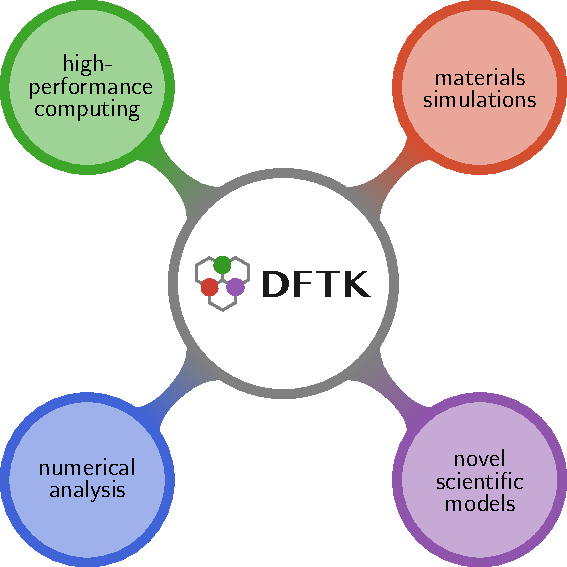
\includegraphics[width=4.6cm]{dftk.pdf}}
    \caption{The multidisciplinary
        directions of research in density-functional theory
        for which DFTK provides a joint software platform.}
    \label{fig:logodftk}
\end{figure}
\section{Acknowledgements} This project has received funding from the institute of
computing and data sciences (ISCD, Sorbonne Université), École des Ponts
ParisTech, Inria Research Centre Paris and from the European Research Council
(ERC) under the European Union's Horizon 2020 research and innovation program
(grant agreement No 810367).

\bibliographystyle{juliacon}
\bibliography{ref}

% \vadjust{\vfill\pagebreak}
\end{document}
